\documentclass{handout}

% \SetInstructor{Lt Col James Phillips}
\SetCourseTitle{ECE231: Electrical Circuits and Systems I}
\SetSemester{Spring 2016}
\SetHandoutTitle{Lecture 19: Time Varying Signals}

%\SetDueDate{1 Jan 2016}
%\ShowAllBlanks

\showsoln \setsolncolor{red}

\begin{document}
\maketitle

\textbf{OBJECTIVES:}
\begin{enumerate}
\item Understand and be able to use the unit step function
\item Understand and be able to use the unit ramp function
\item Understand and be able to use the delta function
\item Understand and be able to use  exponential functions
\item Understand and be able to use sinusoidal functions
\end{enumerate}

\textbf{READING}
\begin{description}
\item [Required]:
\begin{itemize}
\item  Textbook, section 5.1--5.5, pages 240--261
\end{itemize}
\item [Optional]: None
\end{description}

\section{Introduction to time varying signals}
Until now, we have been looking only at signals (voltage, current) that are constant for all time.  They were at a give value prior to our circuit analysis and will remain at the value throughout our analysis.  Moving forward, we will need to look at some time varying signals.  Specifically we will look at the following signals:

\soln{3in}{
\begin{enumerate}
\item Unit Step function
\item Delta function (or impulse function)
\item Ramp function
\item Exponential function
\item Sinusoids
\end{enumerate}
}

We will also show how these waveforms can be combined to synthesize more complex waveforms.

\newpage
\clearpage
\pagebreak

\section{The Unit Step Function}
We start with the simplest of our new signals.  The unit step function is simply zero before time $t<0$ and equal to 1 for time $t\ge0$.  Mathematically,
\soln{1in}{
\begin{equation}
u(t) =
\begin{cases}
0 &\text{for $t<0$}\\
1 &\text{for $t\ge0$}
\end{cases}
\end{equation}
}
The unit step function is shown in Figure \ref{fig: UnitStep}.
\begin{figure} [h!]
\centering
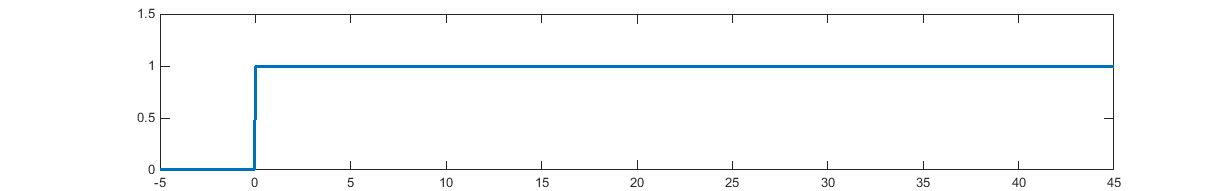
\includegraphics[width=0.9\textwidth]{UnitStep.jpg}
\caption{Unit Step Function}
\label{fig: UnitStep}
\end{figure}

\textbf{Example 1 - Scaling of the unit step} -- Draw a graph of $5u(t)$

\soln{4in}{
First graph $u(t)$
\begin{figure} [h!]
\centering
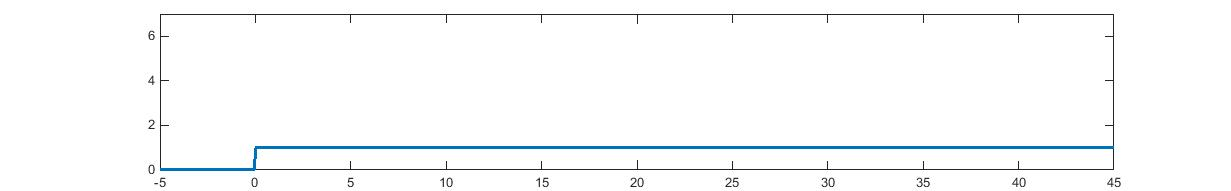
\includegraphics[width=0.9\textwidth]{UnitStepGraph.jpg}
\end{figure}

Multiply entire graph by 5
\begin{figure} [h!]
\centering
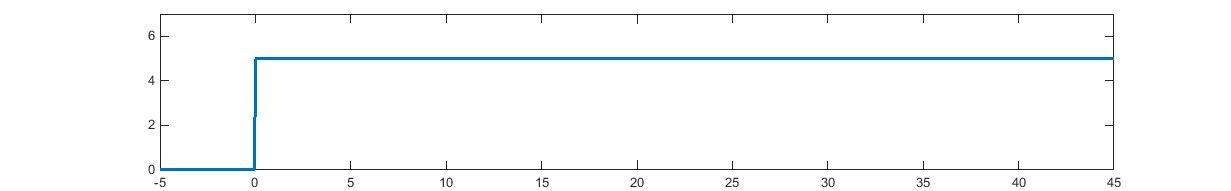
\includegraphics[width=0.9\textwidth]{UnitStepGraph_times_5.jpg}
\end{figure}

}

\textbf{Shifting the unit step--}  What if I want the step function to turn on at some time other than $t=0$? The unit step function always turns on when the arguement is equal to zero.  What if I replace the arguement $t$ with $t - t_0$? It should be obvious that $t-t_0=0$ only when $t=t_0$.

\newpage
\clearpage
\pagebreak

\textbf{Example 2 - Shifting the unit step} -- Graph $u(t-10)$

\soln{2in}{
The arguement of this step function equals zero when $t = 10$
\begin{figure} [h!]
\centering
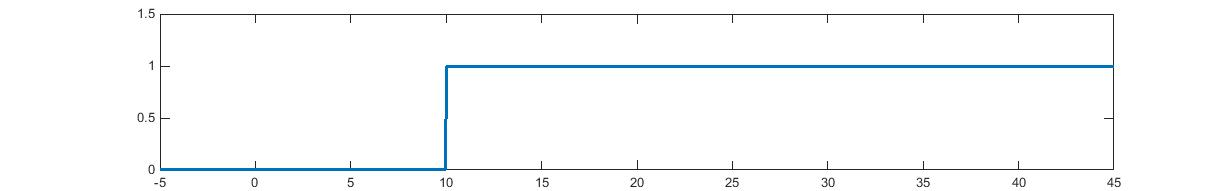
\includegraphics[width=0.9\textwidth]{ShiftedUnitStepGraph.jpg}
\end{figure}
}


\textbf{Adding and subtracting unit step functions}--Next we will look at adding and subtracting shifted and scaled step funtions to create composite functions.

\textbf{Example 3 - Creating a pulse}--Can we write an equation for a single pulse with amplitude 2.  The pulse should be on for $8s\le t\le 15s$.

\soln{6in}{
To start lets write an equation for an amplitude $2$ step function that turns on at 8 seconds.
\begin{equation}
f(t) = 2u(t-8)
\end{equation}
Now we can write an equation for an ampitude $-2$ step function that starts at 15 seconds
\begin{equation}
f(t) = -2u(t-15)
\end{equation}
What if we add these?
\begin{equation}
f(t) = 2u(t-8)-2u(t-15)
\end{equation}
The result is shown in the graph below:
\begin{figure} [h!]
\centering
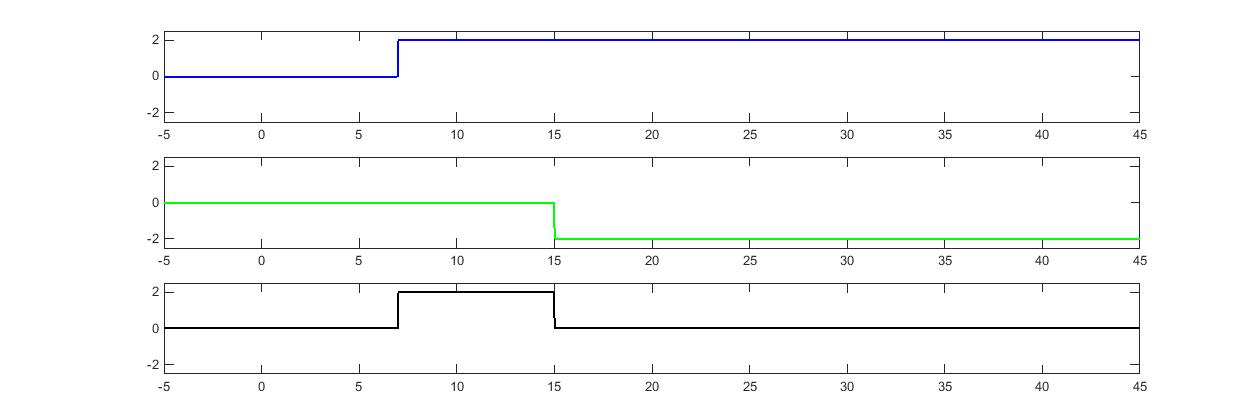
\includegraphics[width=0.9\textwidth]{Example3.jpg}
\end{figure}
}

\newpage
\clearpage
\pagebreak

\textbf{Example 4}--Using step functions, write an equation for the plot shown in Figure \ref{fig: Example4}.
\begin{figure} [h!]
\centering
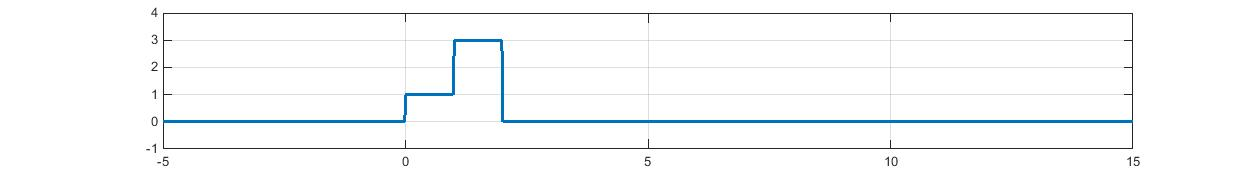
\includegraphics[width=0.9\textwidth]{Example4.jpg}
\caption{Plot for Example 4}
\label{fig: Example4}
\end{figure}

\soln{3in}{
The function turns on with a value of 1 at $t=0$
\begin{equation}
f(t) = u(t)
\end{equation}
At time $t=1$ the value of the function increases to 3 (an increase of 2)
\begin{equation}
f(t) = u(t) + 2u(t-1)
\end{equation}
Finally the function turns off at time $t = 2$, (a decrease of 3)
\begin{equation}
f(t) = u(t)+2u(t-1) -3u(t-2)
\end{equation}
}

\newpage
\clearpage
\pagebreak

\section{The Unit Ramp Function}
The unit ramp function is defined as
\begin{equation}
r(t) = tu(t)
\end{equation}
which can be expanded (for clarity)
\soln{1.5in}{
\begin{equation}
r(t) =
\begin{cases}
0 &\text{for $t<0$}\\
t &\text{for $t\ge0$}
\end{cases}
\end{equation}
}
It should be obvious that this function (for positive $t$) is just a ramp with $slope=1$. The unit ramp is shown in Figure \ref{fig: Ramp}
\begin{figure} [h!]
\centering
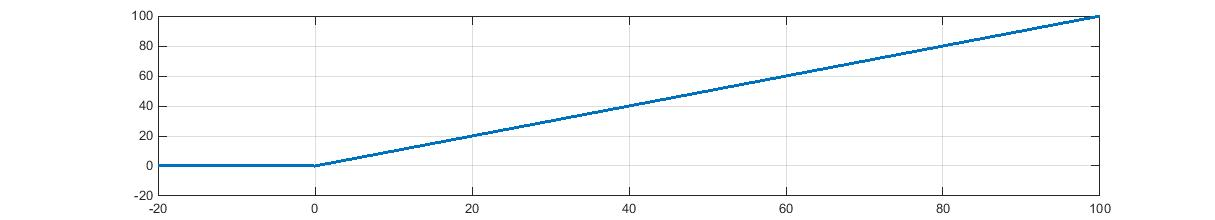
\includegraphics[width=0.9\textwidth]{ramp.jpg}
\caption{The Unit Ramp}
\label{fig: Ramp}
\end{figure}

\textbf{What happens if we multiply the unit ramp by a scalar?}

\soln{1.5in}{
\begin{equation}
A\times r(t) =
\begin{cases}
A \times 0  = 0 &\text{for $t<0$}\\
A \times t = At &\text{for $t\ge0$}
\end{cases}
\end{equation}
We change the slope for $t>0$.  See figure below to see $r(t)$ and $5r(t)$ on the same graph
\begin{figure} [h!]
\centering
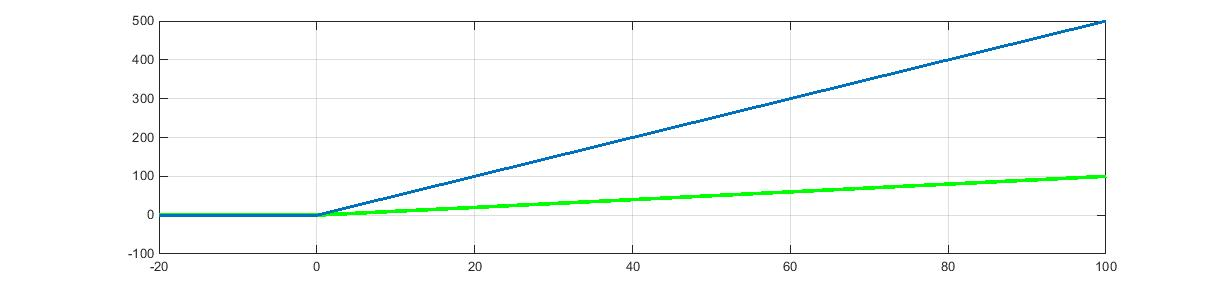
\includegraphics[width=0.9\textwidth]{ScaledRamp.jpg}
\end{figure}
}

\textbf{Can we shift a ramp function?}

\soln{1.5in}{
Yes!, just like we shift a unit step
\begin{equation}
r(t-t_0) =
\begin{cases}
0 &\text{for $t<t_0$}\\
t-t_0 &\text{for $t\ge t_0$}
\end{cases}
\end{equation}
}

It should also be clear that you can combine the two properties above to get a shifted and scaled ramp
\soln{1.5in}{

\begin{equation}
Ar(t-t_0) =
\begin{cases}
0 &\text{for $t<t_0$}\\
A(t-t_0) &\text{for $t\ge t_0$}
\end{cases}
\end{equation}
}

\newpage
\clearpage
\pagebreak

\section{Delta (or impulse) Function}
To understand an impulse function, lets start by writing an equation of a unit area pulse centered on $t=0$
\begin{equation}
\delta (t) = \frac{1}{T}\left[u(t+\frac{T}{2}) -u(t-\frac{T}{2})  \right]
\end{equation}
What happens if we take the limit of this function as $T\rightarrow 0$?

\soln{1in}{
The pulse getters narrower and the amplitude gets higher, but the area always stays 1.  In the limit you have a zero width pulse with inifinite amplitude and area 1.  Mathematicians will have to forgive me..... We call this a delta function.

Mathematically
\begin{equation}
\delta (t) =
\begin{cases}
0 &\text{for $t\neq 0$}\\
\infty &\text{for $t=0$}
\end{cases}
\end{equation}
}

It should also be noted that the delta function is related to the unit step by
\begin{equation}
\delta (t) = \frac{\partial u(t)}{\partial t}
\end{equation}

Since this function is related to the unit step and the unit step can be shifted, so can the delta function.
\soln{2in}{
\begin{equation}
\delta (t-t_0) =
\begin{cases}
0 &\text{for $t\neq t_0$}\\
\infty &\text{for $t=t_0$}
\end{cases}
\end{equation}
}

\newpage
\clearpage
\pagebreak

\section{Exponential Functions}
Pay attention to this section... Exponential functions are important in circuit analysis...

An exponential function has the form
\soln{1.2in}{
\begin{equation}
f(t) = e^{-(t-t_0)}u(t-t_0)
\end{equation}

Note: Because of the step function it is always zero prior to $t=t_0$
}

For $t_0 =0$ this simplfies to
\soln{1.2in}{
\begin{equation}
f(t) = e^{-t}u(t)
\end{equation}
}

The plot of this function is shown in Figure \ref{fig: Exponential}
\begin{figure} [h!]
\centering
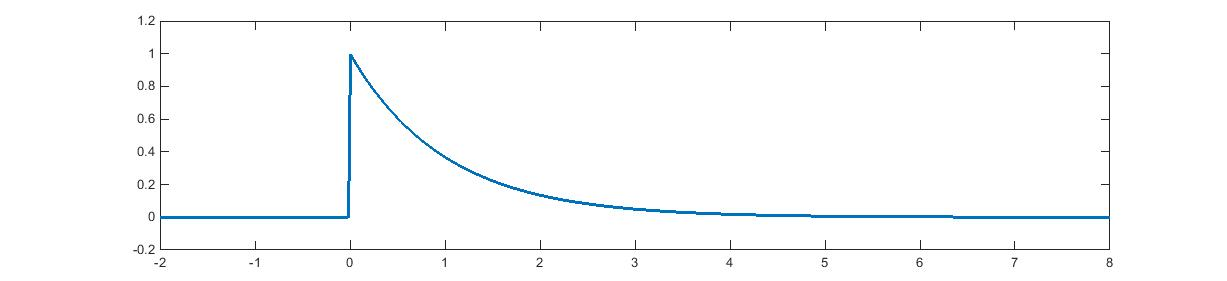
\includegraphics[width=1\textwidth]{Exponential.jpg}
\caption{Exponential Function}
\label{fig: Exponential}
\end{figure}

\textbf{Does this function ever reach zero?}
\soln{1.2in}{
No, but it will get very close.... As a matter of fact when it reaches $0.67 \%$ we will say it is effectively zero.
}

\textbf{How long does it take to decay to this value?} -- To really talk about the decay time we have to modify our equation a little and introduce the concept of a time constant , $T_c$.  If we include the time constant our equation now looks like
\soln{1.2in}{
\begin{equation}
f(t) = e^{-\frac{t}{T_c}}u(t)
\end{equation}

Note: It should be obvious in our simple form of the equation from before $T_c=1$
}

To find out how fast this function decays, lets calculate the value of $f(t)$ for different values of $t$

\soln{3in}{
The table below shows the value of $f(t)$ after integer numbers of time constants have passed.
\begin{table}[h]
\centering
\begin{tabular}{|c|c|}
\hline
$t$ & $f(t)$  \\
\hline \hline
$0$ &  1.000 \\
$1T_c$ &  0.367 \\
$2T_c$  & 0.135 \\
$3T_c$  & 0.049  \\
$4T_c$  & 0.0183 \\
$5T_c$  & 0.0067  \\
\hline
\end{tabular}
\end{table}

This shows that an exponential function is effectively zero after 5 time constants (some texts will use 4 time constants).

}

Much like the unit step function, we can also scale the amplitude of the exponential function.  This gives us:
\soln{1in}{
\begin{equation}
f(t) =A e^{-\frac{t}{T_c}}u(t)
\end{equation}

Where A is the amplitude and $T_c$ is the time constant (as before).
}

 \textbf{Example 5} -- Plot $f(t) = 4e^{-1000t}u(t)$ and determine with the function is effectively equal to zero.

\soln{4in}{
First calculate the time constant:
\begin{equation}
T_c = \frac{1}{1000} = 1\ ms
\end{equation}
This immediately tells us that the function is effectively zero after $5\ ms$.

To plot the function we need to calculate a few values.... We will use our table from before.  We know our inital value is 4 and after 1 $T_c$ the function has decayed to $36.7\%$ of its initial value, and after 2 $T_c$ it has decayed to $13.5\%$, etc

\begin{table}[h]
\centering
\begin{tabular}{|c|c|}
\hline
$t$ & $f(t)$  \\
\hline \hline
$0$ &  1.000 \\
$1\ ms$ &  1.468 \\
$2\ ms$  & 0.540 \\
$3\ ms$  & 0.196  \\
$4\ ms$  & 0.073 \\
$5\ ms$  & $\approx 0$  \\
\hline
\end{tabular}
\end{table}

The plot is shown below:
\begin{figure} [h!]
\centering
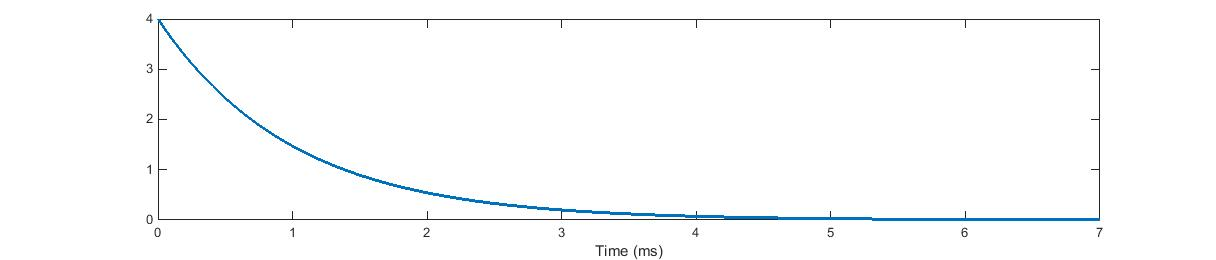
\includegraphics[width=0.9\textwidth]{Example4soln.jpg}
\end{figure}
}

\newpage
\clearpage
\pagebreak

\section{Sinusoids}
Understanding sinusoids is critical to the study of many areas of science and engineering; this is very true in our study of electrical circuits.

Note: All the functions we have defined above are zero for $t<0$; for our sinusoids we will assume they exist for all time, $-\infty<t<\infty$.

\subsection{Sinusoid Basics}

A simple sinusoid can be expressed as either a sine or a cosine function
\soln{1in}{
\begin{eqnarray}
f_1(t) &=&sin\left\{\frac{2\pi  t}{T_0}  \right\} \nonumber \\
f_2(t) &=&cos\left\{\frac{2\pi  t}{T_0}  \right\} \nonumber
\end{eqnarray}
}
where $T_0$ is the period of the sinusoid

Sine and Cosine are shown as funcntions on time in Figure \ref{fig: SinCos_1}
\begin{figure} [h!]
\centering
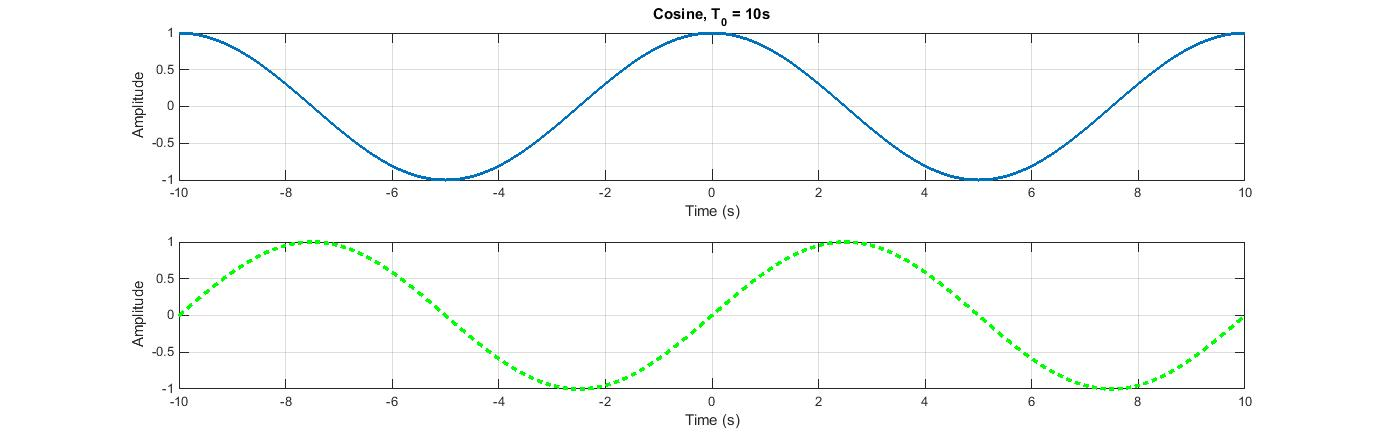
\includegraphics[width=1\textwidth]{SinCos_1.jpg}
\caption{Sin and Cos shown as functions of time}
\label{fig: SinCos_1}
\end{figure}

Another way to view {\em sin} and {\em cos} is to look at them on the same graph as a function of angle.  That is what you see in Figure \ref{fig: SinCos_2}:

\begin{figure} [h!]
\centering
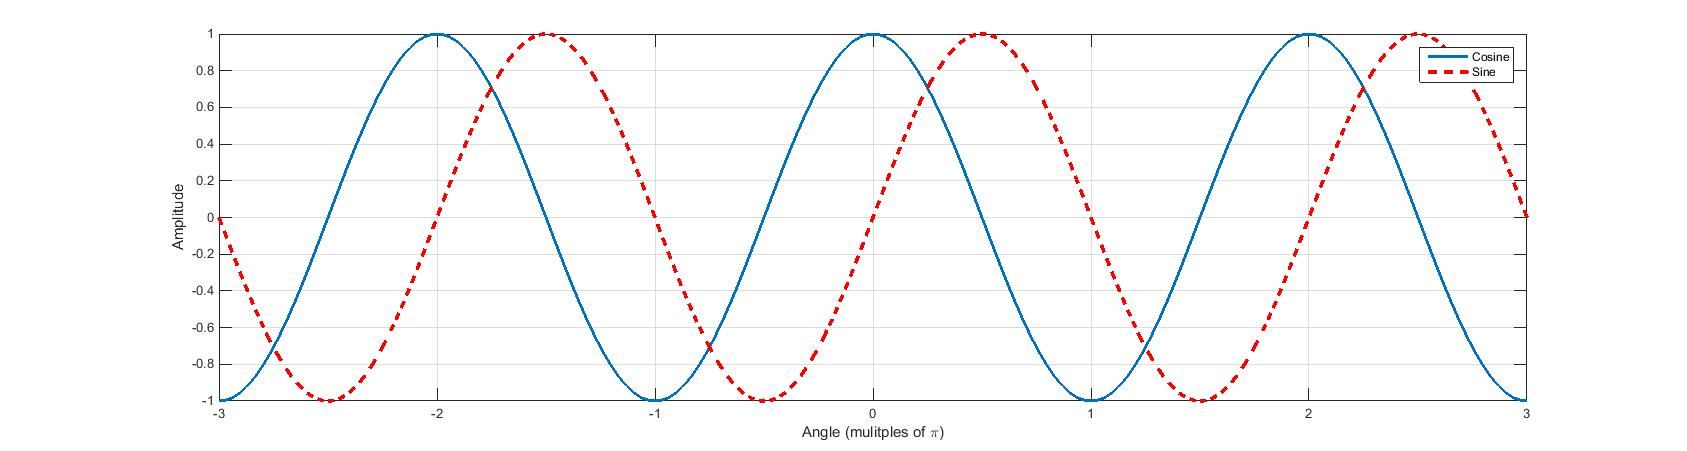
\includegraphics[width=1\textwidth]{SinCos_2.jpg}
\caption{Sin and Cos shown as functions of angle (in multiples of $\pi$)}
\label{fig: SinCos_2}
\end{figure}
What you should notice here is that the cos wave {\em leads} the sin wave by $90 ^\circ$ or $\frac{\pi}{2}\ rad$.  They are otherwise identical.  This can be written mathematically as
\soln{1in}{
\begin{equation}
\cos(\theta) = \sin\left (\theta + \frac{\pi}{2}\right )
\end{equation}
}

\subsection{Time or Phase Shifted Sinusoids}
This section will discuss shifted sinusoids.  Mathematically a phase shifted or time shifted sinusoid are the identical (which we will show).  The text book refers to this as a general sinusoid and it has the form:
\soln{1.5in}{
\begin{equation}
f(t) = A\cos\left\{\frac{2\pi(t-T_s)}{T_0}  \right\}
\end{equation}
where $A$ is the amplitude, $T_0$ is the period (as before) and $T_s$ is the time shift.
}

We can exapand this eqaution to show that the time shift can also be represented as a angular phase shift:
\soln{1.5in}{
\begin{equation}
f(t) = A\cos\left\{\frac{2\pi t}{T_0}-\frac{2\pi T_s}{T_0}  \right\} = A\cos\left\{\frac{2\pi t}{T_0}+\phi \right\}
\end{equation}
is should be evident that
\begin{equation}
\phi = -\frac{2\pi T_s}{T_0}
\end{equation}
$\phi$ is in radians.
}

The phase shift is often displayed in degrees instead of radians:
\soln{1in}{
\begin{equation}
\phi = -\frac{360^\circ T_s}{T_0}
\end{equation}
}

Care must be taken when doing calculations to not mix degrees and radians!

\textbf{Example 6} -- Plot $f(t) = 4\cos(\frac{\pi t}{5} -30 ^\circ)$ as a function of time:

\soln{4in}{
First find the period $T_0$:
\begin{equation}
\frac{2\pi t}{T_0} = \frac{\pi t}{5}
\end{equation}
Therefore $T_0= 10\ s$

Next, convert $30^\circ$ to $rad$:
\begin{equation}
-30^\circ *\frac{\pi}{180^\circ} = -\frac{\pi}{6}
\end{equation}

Next we can convert $\phi$ to a time shift $T_s$ (remember $T_0=10$):
\begin{equation}
-\frac{2\pi T_s}{T_0} = -\frac{2\pi T_s}{10}=-\frac{\pi}{6}
\end{equation}
Therefore $T_s=1.2s$

So we have a cosine with $A = 4$, $T_0=10s$ and $T_s = 1.2s$:
\begin{figure} [h!]
\centering
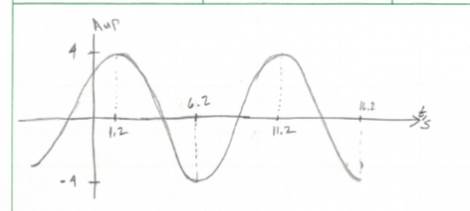
\includegraphics[width=0.7\textwidth]{Example6soln.jpg}
\end{figure}
}
\newpage
\clearpage
\pagebreak

An alternative version of a general sinusoid can be derived by starting with:
\begin{equation}
f(t) =  A\cos\left\{\frac{2\pi t}{T_0}+\phi \right\}
\end{equation}
and expanding it using the following trigonometric identity:
\begin{equation}
\cos(x +y) = \cos(x)\cos(y)-sin(x)sin(y)
\end{equation}
I will leave the algebra to you, but using the last two equations we can arrive at
\begin{equation}
f(t) = A\cos \phi \cos \left(\frac{2\pi t}{T_0}\right)-A \sin \phi \sin \left(\frac{2\pi t}{T_0}\right)
\end{equation}
$A\cos\phi$ and $A\sin\phi$ are constants and are referred to as Fourier coefficients.


\subsection{Damped Sinusoids}
The last functions we will discuss are damped sinusoids; these functions are the product of a decaying exponential and a sinusoid and have the form

\soln{1.5in}{
\begin{equation}
f(t) = Ae^{-\alpha t}\cos\left\{\frac{\beta t}{T_0}  \right\}
\end{equation}
where we have neglected any time shifts and $\alpha$ is an attenuation constant (or $\frac{1}{T_c}$) and $\beta = \frac{2\pi}{T_0}$
}

To graph a damped sinusoid graph the decaying exponential, then mirror is across the $t$ axis, then fill it in with the appropriate sinusoid.

\textbf{Example 7} -- Graph $f(t) = 5e^{5t}\cos\left(20\pi t  \right)$

\soln{4in}{
\begin{figure} [h!]
\centering
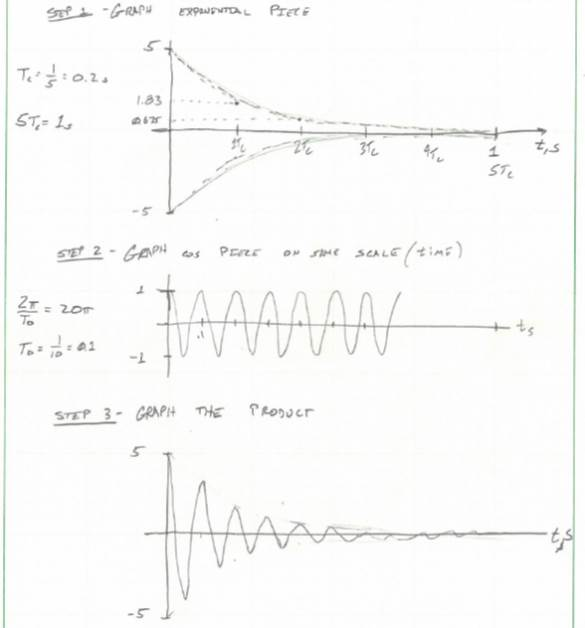
\includegraphics[width=0.6\textwidth]{Example7soln.jpg}
\end{figure}

OR USE MATLAB!
}
\newpage
\clearpage
\pagebreak

\newpage
\clearpage
\pagebreak

\newpage
\clearpage
\pagebreak

\newpage
\clearpage
\pagebreak

\newpage
\clearpage
\pagebreak

\newpage
\clearpage
\pagebreak

\newpage
\clearpage
\pagebreak

\end{document}


% Equation Array Example Code
%\begin
%{eqnarray}
%P_R &=& i_R^2R \nonumber \\
%P_R &=& (100\ mA)^2 \times 100\ \Omega \nonumber \\
%P_R &=& (100 \times 10^{-3}\ A)^2 \times 100\ \Omega \\
%P_R &=& 10000 \times 10^{-6}\ A^2  \times 100\ \Omega \nonumber \\
%P_R &=& 1\ W  \nonumber
%\end{eqnarray}

% Figure Example Code
%\begin{figure} [h!]
%\centering
%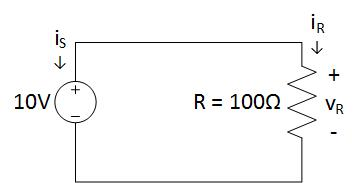
\includegraphics[width=0.5\textwidth]{OhmsLawExampleSolution.jpg}
%\caption{Ohm's Law example circuit}
%\label{fig: OhmsLawExampleSolution}
%\end{figure}

%Table Example Code
%\begin{table}[h]
%\centering
%\begin{tabular}{|l|c|c|}
%\hline
%Prefix & Abbreviation & Value \\
%\hline \hline
%Giga & $G$ & $10^9$ \\
%Mega & $M$ & $10^6$ \\
%Kilo & $k$ & $10^3$ \\
%\hline
%milli & $m$ & $10^{-3}$ \\
%micro & $\mu$ & $10^{-6}$ \\
%nano & $n$ & $10^{-9}$ \\
%pico & $p$ & $10^{-12}$ \\
%\hline
%\end{tabular}
%\caption{Engineering prefixes and values}
%\label{tab: Eng Prefixes}
%\end{table}
